\documentclass[10pt,a4paper,twocolumn]{article}
\usepackage[margin=19mm,columnsep=6mm]{geometry}
\usepackage[T1]{fontenc}
\usepackage{lmodern}
\usepackage{microtype,amsmath,amssymb,graphicx,booktabs,longtable,array}
\usepackage[numbers,sort&compress]{natbib}
\usepackage[colorlinks=true,linkcolor=blue,citecolor=blue,urlcolor=blue]{hyperref}
\usepackage{caption,fancyhdr,float}
\usepackage{dblfloatfix}
\usepackage{listings}
\lstset{basicstyle=\ttfamily\footnotesize,breaklines=true,columns=fullflexible,
  keepspaces=true,showstringspaces=false,frame=single,aboveskip=5pt,belowskip=5pt}
\setcounter{dbltopnumber}{2}
\renewcommand{\dbltopfraction}{.9}
\renewcommand{\textfraction}{.05}
\renewcommand{\dblfloatpagefraction}{.8}
\graphicspath{{../figures/}}
\captionsetup{font=small,labelfont=bf}
\setlength{\parskip}{3pt}
\setlength{\parindent}{1em}
\setlength{\textfloatsep}{12pt}
\setlength{\floatsep}{9pt}
\pagestyle{fancy}
\fancyhf{}
\fancyhead[L]{\small Memory Under Interference}
\fancyhead[R]{\small Preprint -- Version 1.0}
\fancyfoot[C]{\thepage}
\setlength{\headheight}{14pt}
\newcommand{\MainRequests}{5,528}
\newcommand{\SmallCross}{3.12}
\newcommand{\SmallCrossCI}{[-3.12, 11.25]}
\newcommand{\SmallCrossN}{40}
\newcommand{\SmallCrossP}{1}
\newcommand{\SmallFullEnergy}{325.38}
\newcommand{\SmallOracleEnergy}{76.39}
\newcommand{\SmallEnergyDiff}{-249.00}
\newcommand{\SmallEnergyCI}{[-529.62, -127.49]}
\newcommand{\SmallPromptDiff}{-2.25}
\newcommand{\SmallPromptCI}{[-7.77, 2.86]}
\newcommand{\SmallPromptP}{0.44696}
\newcommand{\SmallInitialDiff}{-27.50}
\newcommand{\SmallInitialCI}{[-45.00, -10.00]}
\newcommand{\SmallInitialP}{0.033691}
\newcommand{\SmallTargetDiff}{-11.25}
\newcommand{\SmallTargetCI}{[-20.62, -2.50]}
\newcommand{\SmallTargetP}{0.056396}
\newcommand{\LargeCross}{8.97}
\newcommand{\LargeCrossCI}{[3.21, 16.67]}
\newcommand{\LargeCrossN}{39}
\newcommand{\LargeCrossP}{0.03125}
\newcommand{\LargeFullEnergy}{154.16}
\newcommand{\LargeOracleEnergy}{50.20}
\newcommand{\LargeEnergyDiff}{-103.96}
\newcommand{\LargeEnergyCI}{[-152.30, -77.58]}
\newcommand{\LargePromptDiff}{2.64}
\newcommand{\LargePromptCI}{[-1.22, 6.30]}
\newcommand{\LargePromptP}{0.44156}
\newcommand{\LargeInitialDiff}{-2.50}
\newcommand{\LargeInitialCI}{[-17.50, 12.50]}
\newcommand{\LargeInitialP}{1}
\newcommand{\LargeTargetDiff}{-2.50}
\newcommand{\LargeTargetCI}{[-10.00, 4.39]}
\newcommand{\LargeTargetP}{0.63525}
\newcommand{\EmbeddingMRR}{0.7364}
\newcommand{\LexicalMRR}{0.5163}

\title{\vspace{-1cm}Memory Under Interference:\\Context Utilization, Specification Confusion, and Inference Efficiency in Small Code Language Models}
\author{Dhruv Brahmbhatt\\\normalsize IIT Madras student; independent researcher\thanks{This independent study is not presented as sponsored, supervised or endorsed by IIT Madras.}}
\date{24 November 2026\\[3pt]\small Preprint -- Version 1.0 -- Not peer reviewed}

\begin{document}
\maketitle
\begin{abstract}
Relevant information can be present in a language model's context while its
generated code follows a competing requirement. We investigate this gap in two
small quantized Qwen2.5-Coder models on one CPU laptop. Seven completed studies
contain \MainRequests{} main-study logical requests, including documented
failures; pilots and an incomplete cache study remain separate. Controlled
contexts vary task load, competing specifications, static interruptions,
retention policies and a code-only preference. Cross-specification evaluation
tests saved programs against both target and alternative requirements. In a
posthoc paired analysis, the 1.5B model has \LargeCross{} percentage points more
alternative-consistent failures under competing than irrelevant context
(95\% task-bootstrap interval \LargeCrossCI{}; \LargeCrossN{} matched tasks).
The 0.5B result is inconclusive, and adverse coding of censored outcomes weakens
the 1.5B finding. Relative to full history, oracle retention has observed
estimated net CPU-package energy-per-correct-solution reductions of
\SmallEnergyReduction\% and \LargeEnergyReduction\% for 0.5B and 1.5B.
Accuracy preservation is uncertain; length, position, instructions and output
work differ, so these reductions cannot be attributed exclusively to retention.
A registered preference metric reaches a floor that a separate format audit
helps explain. MemoryGraph is a companion retrieval prototype with a separate
synthetic evaluation, not an evaluated intervention in these studies. Together,
the results motivate testing what retrieved context makes a system do, alongside
what it retrieves and what inference costs.
\end{abstract}

\section{Introduction}
Memory-management systems decide which past instructions, preferences and task
descriptions to put in a model's next prompt. More context can preserve useful
information, but it can also keep obsolete or competing requirements in view.
For a coding assistant, the consequence may be a program that is sensible for
the wrong specification. A useful evaluation must therefore connect context
selection to executable behavior and computational cost, rather than judge
success from the presence of relevant text alone.

Prior work already shows position-sensitive context use, conversational task
interference, and difficulty following user preferences
\citep{lost,interference,prefeval}. Multi-task inference can also help some
tasks \citep{multitask}; degradation is not a universal consequence of bundling.
We examine these established concerns in two small local code models, using
execution-based outcomes and CPU-package measurements on consumer hardware.

Three research questions organize the report. \textbf{RQ1:} How does task-bearing
context compare with length-matched neutral material? \textbf{RQ2:} Are target
failures more often consistent with a competing specification when that
specification appears in context? \textbf{RQ3:} How do retention and preference
policies relate to correctness and inference cost? These are questions about
observable programs, not internal memory capacity or cognitive states.

\paragraph{Contributions.}
We provide (1) a controlled contextual-interference evaluation with paired
code tasks, matched controls and distinct task-load/interruption constructions;
(2) a cross-specification failure diagnosis that separates target-only,
alternative-only, both-pass and neither-pass outcomes, with isolation
cross-scoring and posthoc censoring analyses; and (3) an evaluation of
context-retention correctness and computational-efficiency trade-offs that
includes failed-attempt cost and uncertainty in cost per correct solution.
Sanitized journals, exact prompts and portable analysis accompany the report.

The findings are mixed. Competing context changes the larger model's observed
error distribution in the complete cases, but censoring weakens the inference.
Oracle retention has lower observed estimated costs, without established
accuracy preservation. A preference-scoring floor and several null comparisons
show where the evidence is less informative. The seven-study collection grew
from Prompt-Energy through dated design revisions; registered comparisons and
posthoc analyses remain distinguished throughout. The separate MemoryGraph
prototype connects these questions to practical retrieval without supplying
an integrated performance claim.

\section{Related Work}
\paragraph{Context and instruction interference.}
Lost in the Middle studies relevant-information position in question answering
and retrieval \citep{lost}. Gupta et al. examine task switches in conversation
history \citep{interference}; our static interruption study is closely related,
but does not contain actual preceding model task execution. Son et al. find
that multi-task inference can improve performance and speed on their benchmark
\citep{multitask}. Our much smaller code models and different tasks do not
contradict that result merely because some bundled conditions perform worse.
Instruction Hierarchy addresses conflicting privilege levels and training for
robust prioritization \citep{hierarchy}. We neither train a hierarchy nor
evaluate adversarial security robustness.

\paragraph{Memory and preferences.}
PrefEval examines explicit and implicit preference following in longer
conversations \citep{prefeval}; our code-only preference and mechanical metric
are a much narrower instrument. LongMemEval separates indexing, retrieval and
reading in conversational memory systems \citep{longmem}. Recent EvalMem
explicitly diagnoses encoding, retrieval and generation defects
\citep{evalmem}, while LongMemEval-V2 examines experience-oriented agent memory
\citep{longmemv2}. Thus, separating availability from retrieval and generation
is not itself a novelty claim. Our main studies do not implement a memory store
or diagnose encoding defects; they test already-rendered code-task contexts.

\paragraph{Code evaluation and efficiency.}
HumanEval introduced execution-based code-generation evaluation
\citep{humaneval}; EvalPlus expands its tests and demonstrates the consequences
of insufficient oracles \citep{evalplus}. Qwen2.5-Coder supplies the model
family \citep{qwen}. Prior inference-energy benchmarking relates cost to
outputs, prompts and runtime settings \citep{sustainable}. A directly
overlapping 2026 study evaluates prompting, code accuracy and environmental
cost across small/open models \citep{slmenergy}. We do not claim the first
prompt-energy study, nor transfer its hardware or carbon results to this laptop.

\paragraph{Practical retrieval.}
GraphRAG builds graph indexes and community summaries for corpus-level
questions \citep{graphrag}; Mem0 studies a more integrated persistent-memory
system \citep{mem0}. Our companion MemoryGraph implements far less. Its small
entity graph and synthetic retrieval results motivate a future bridge, not a
claim of equivalent architecture or evaluated user benefit. The release's
related-work table records each publication's design, overlap and the limited
distinction supported here. This is a focused review, not an exhaustive search
or proof of priority.

\section{Evaluation Framework}
We distinguish four operations. \emph{Availability} means that the intended
specification is literally present in the rendered prompt. \emph{Retrieval}
means selecting stored material for a prompt; it is only demonstrated in the
separate companion prototype. \emph{Utilization} is operationalized by the
generated function's observed test outcomes. \emph{Efficiency} describes
measured tokens, latency and qualified CPU-package estimates, including failed
attempts. None is a direct measurement of internal memory capacity.

For a target program test suite $T$ and a corresponding computational
alternative $A$, an uncensored response belongs to one of four cells:
target-only pass, alternative-only pass, both pass, or both fail. We call the
second cell \emph{alternative-consistent} or \emph{distractor-only} success.
``Specification confusion'' in the title refers only to this operational error
pattern. Passing a finite suite does not prove general program correctness,
and a different failure may reflect syntax, extraction, policy restrictions or
ordinary algorithmic error.

\begin{figure*}[t]
\centering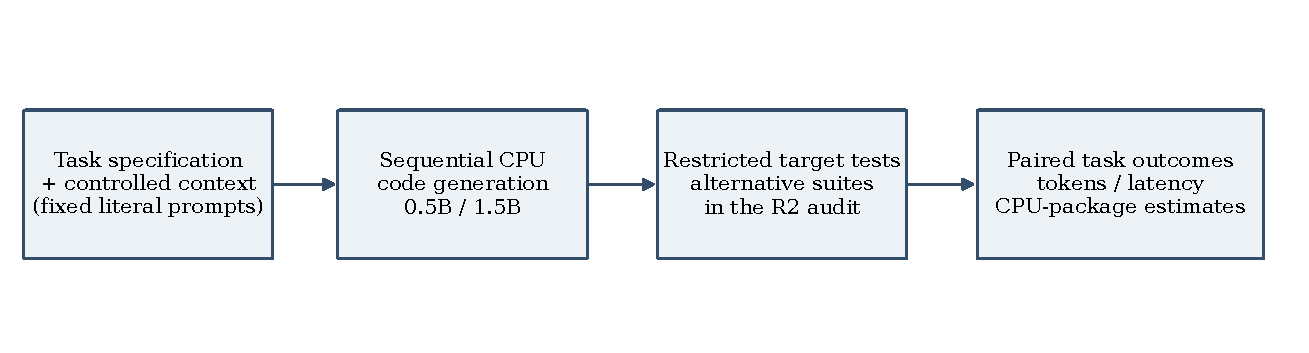
\includegraphics[width=\linewidth]{framework.pdf}
\caption{Observed-data framework. Target and context text are frozen before
generation. Scoring is separate and restricted. The additional alternative-suite
analysis uses saved outputs; it does not generate new answers.}
\label{fig:framework}
\end{figure*}

For each model and paired task $t$, let $y_{tc}$ denote a binary test outcome,
or the mean over the registered repeated cells in condition $c$. We report
$\widehat\Delta=|S|^{-1}\sum_{t\in S}(y_{ta}-y_{tb})$, preserving both arms
and all included cells within each resampled task. For energy, the observed
covered-population ratio is
\begin{equation}
\widehat C_c=\frac{\sum_{i\in I_c}E_i}{\sum_{i\in I_c}\mathbf{1}\{\text{correct}_i\}},
\end{equation}
where $I_c$ contains attempts with both energy and correctness readings. Failed
attempts contribute energy to the numerator. We attach coverage and the correct
denominator rather than mix an available-only energy total with all-arm passes.

\section{Experimental Methodology}
\subsection{Data, runtime and actual study scope}
The models are \texttt{qwen2.5-coder:0.5b} and
\texttt{qwen2.5-coder:1.5b}, both Q4\_K\_M quantizations, with exact model
digests recorded in frozen jobs. Inference used Ollama on Windows 11, an Intel
i5-13420H CPU and approximately 16 GB RAM, with eight inference threads and
\texttt{num\_gpu=0}. Generation was sequential, with randomized interleaved
condition schedules. Recorded block-start checks observed AC power and Best
performance; these snapshots do not prove an invariant host state throughout
every request. Decoding settings, templates, native token counts, raw outputs
and retry records are retained.

The main request counts are: isolated strategy comparison, 1,968; initial
context load plus its isolation controls, 280; task bundles, 1,040; retention,
400; revised semantic interference plus isolation, 1,040; static interruptions
plus isolation, 400; and preference placement, 400. These sum directly to
\MainRequests{}. Pilots are separate observations. The revised cache study
saved 76 of 400 planned full requests and is a partial appendix diagnostic.
Repair and recognition/hint studies were not conducted.

The isolated strategy study covers all 164 HumanEval+ tasks, comparing P1 and
P3\_1 with three temperature-0.2 samples per task/model, context 8,192 and output
budget 2,048. The strategies differ in both instructions and an external
example, so this is not a pure example-effect contrast. Initial context load
uses 20 held-out-eligible tasks per model, with fresh temperature-0
no-filler outcomes; the sample used for selection is never the isolation
comparator. Its model-selected populations and weaker renamed-specification
distractors remain separate from the revised designs.

The later studies use the original fixed 40-task roster for both models. They
use temperature 0 and one generation per task-condition-model. Context is
32,768 for task bundles, 16,384 for retention/revised interference/interruptions,
and 8,192 for preferences. Output budgets are 2,048 except that active bundles
receive 2,048 per requested function. Explicit context reservations and native
prompt counts detect mismatches; invalid calls are reported, not repaired by
silent parameter changes.

\subsection{Controlled context constructions}
Passive task load adds other task descriptions; active load requests their
functions as well. $K\in\{2,3,4,6\}$; neutral filler matches passive input
length. Target placement and companions are fixed. Active requests do more
output work, so focal-target, per-function and whole-bundle endpoints are kept
distinct. Reused component-isolation outputs are lookup references, not newly
measured bundle execution.

Revised semantic interference crosses three filler types, filler-token targets
1,000/2,000 and target beginning/end, with matched isolation controls. Competing
descriptions change a computational requirement, such as strict versus
non-strict comparison or inclusive versus exclusive boundaries. Alternative
references and distinguishing inputs were validated. The model sees descriptions,
not the alternative implementation or hidden tests. Related/irrelevant labels
are authored coarse categories; they are not calibrated semantic similarity.
Filler budgets do not guarantee identical complete input lengths across every
wrapper, an important limit on attributing differences solely to content.

Retention compares full history, target/query only, verbatim target replay,
lossless target-format compaction, and oracle retention. Eight fixed distractor
descriptions form full history. No-history omits the explicit code-only
preference, while the oracle retains target, preference and final query.
Compaction removes redundant target formatting and drops other history; it is
not semantic summarization of a conversation. These policies jointly change
length, position, repetition and sometimes instruction content.

Static interruption conditions contain neutral material, one similar competing
description, one other-domain description, or three other-domain descriptions.
Loaded complete input counts match, with the same target and final instruction.
Descriptions and acknowledgements are literal transcripts, not tasks executed
earlier by the model. Similarity, count and diversity are not fully crossed.
Preference placement compares absent, immediate, buried, replayed and corrected
code-only instructions while preserving the target/query and distractor history.

\subsection{Statistics, exclusions and energy}
Intervals use 2,000 paired task-bootstrap draws with seed 1732. Binary pairs use
exact discordant-pair McNemar tests; task means over repeated cells use exact
paired sign swaps. Holm correction is within specified families: two isolated
strategy tests, two initial-load primary tests, two revised-interference primary
tests, six retention tests and six interruption tests. The new cross-pass audit
uses four posthoc tests. These corrections do not control every analysis ever
examined in the project. Intervals are pointwise, not simultaneous family
intervals. Null tests do not establish equivalent accuracy.

The audit preserves failed requests and capped generations. Caps are nonpasses
for bounded correctness endpoints but unknown for the uncensored cross-pass
taxonomy. API, input or evaluator-infrastructure failures are missing for
valid-input accuracy and separately reduce operational yield. We report cap
exclusion, optimistic bounded-correctness scenarios, adverse cross-pass coding,
independently labelled eligibility subsets, and exclusion of the documented
HumanEval/32 oracle anomaly. The expanded-test adapter and sandbox restrictions
remain part of the operational outcome, not an infallible correctness oracle.

HWiNFO CPU Package Power was logged at a nominal 500 ms interval. Gross energy
uses trapezoidal integration; net estimates subtract the block-start idle
baseline over the request window. Approximate post-load and total windows are
both retained. End/midpoint subtraction, drift exclusions and short-window
exclusions are secondary sensitivities. Per-condition totals are preferred to
precise interpretations of short individual windows. The registered primary
cache-energy experiment is incomplete; retention energy remains descriptive or
posthoc. No whole-system electricity, carbon, GPU or cloud inference is measured.

\section{Contextual Interference}
\subsection{Context content and additional output work}
Figure~\ref{fig:m1} compares focal-target outcomes under passive, active and
neutral conditions. Passive-minus-filler estimates tend to be negative across
$K$ in this roster, but many adjusted comparisons are inconclusive. The 0.5B
$K=6$ estimate is $-25$ percentage points, conditional interval $[-37.5,-12.5]$,
with Holm $p=0.015625$ in its eight-comparison posthoc family. This single
conditional contrast does not establish a universal multitasking penalty.

Every bundle-membership graph forms one connected component. Anchor-task
bootstrap intervals condition on the fixed companions and cannot estimate
dependence-robust variability from other bundles. Changing $K$ also changes
which companion functions appear. Active per-function fractions and whole-bundle
successes are reported against the same components' isolation outcomes in the
archive, rather than equating a passive focal pass with a complete active bundle.
The additional output budget and repeated component references limit cost
comparisons. This dependence limitation is substantive, not a small-sample
footnote to a population-level claim.

\begin{figure*}[t]
\centering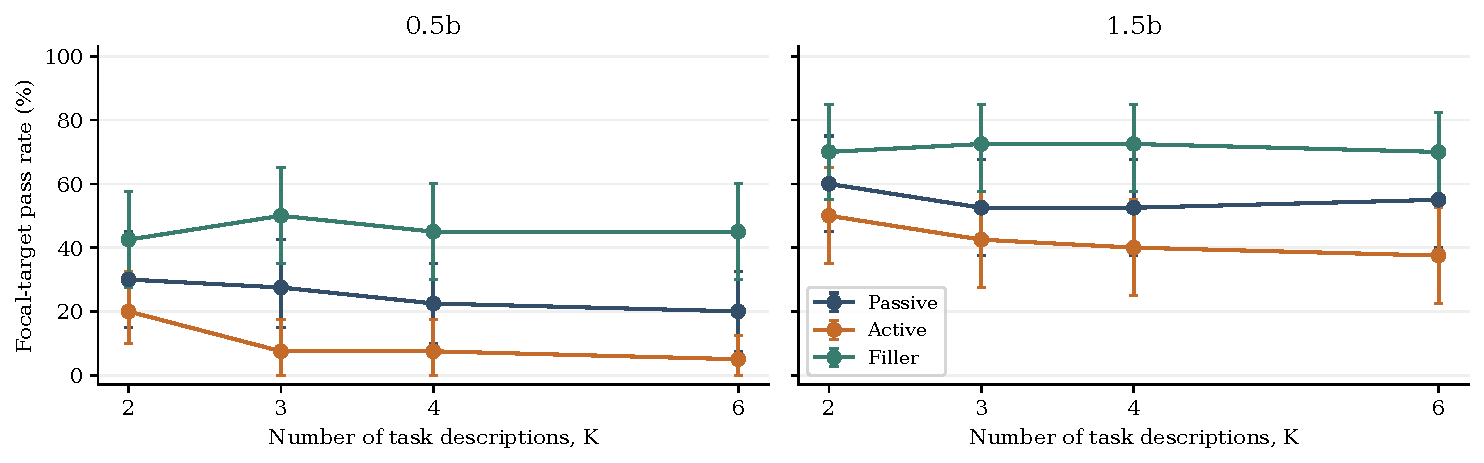
\includegraphics[width=.95\linewidth]{m1.pdf}
\caption{M1 focal-target pass rates, 40 anchors per model/mode/$K$. Whiskers are
conditional task-bootstrap intervals with overlapping fixed companions. Active
mode requests $K$ functions and has a larger output budget. These are not
dependence-robust independent-bundle confidence intervals.}
\label{fig:m1}
\end{figure*}

\subsection{Competing specifications and alternative-consistent failures}
The revised primary competing-minus-irrelevant target-correctness difference is
\SmallTargetDiff{} percentage points for 0.5B, interval \SmallTargetCI{}, Holm
$p=\SmallTargetP{}$, and \LargeTargetDiff{} for 1.5B, interval
\LargeTargetCI{}, Holm $p=\LargeTargetP{}$. Both comparisons have 40 paired
tasks averaged over four length/position cells. A pointwise interval excluding
zero can coexist with an adjusted test that does not reject; both are reported.
Figure~\ref{fig:matrix} shows the cell-level outcomes without treating them as
independent task replications.

\begin{figure*}[t]
\centering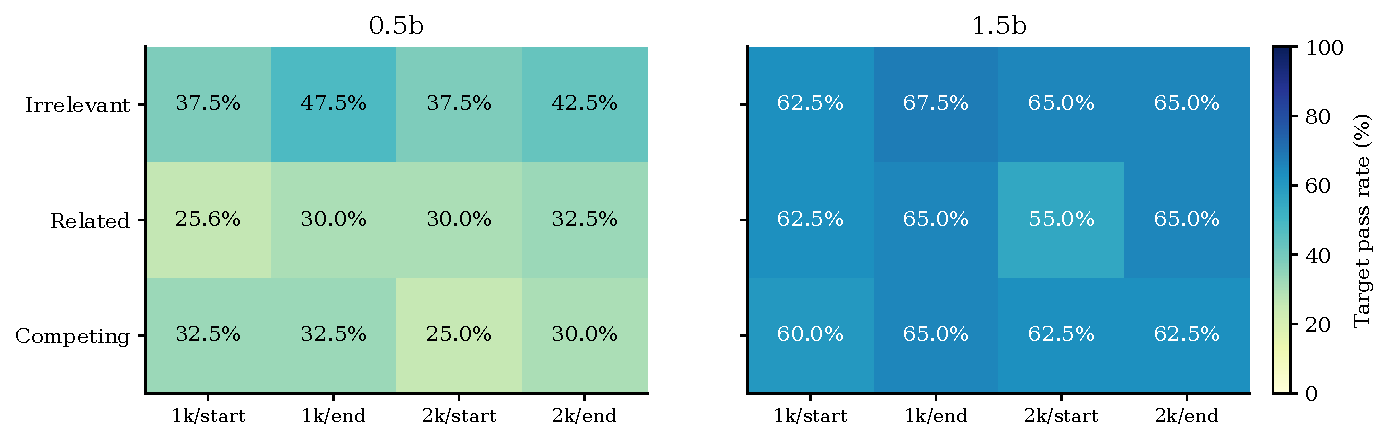
\includegraphics[width=.98\linewidth]{interference_matrix.pdf}
\caption{Revised M3/R2 target pass rates. Columns are filler-token targets and
target positions, not total input length. Cells contain 40 scheduled tasks;
one related-context API failure leaves 39 valid outcomes in its cell. Caps are
bounded-endpoint nonpasses. Per-cell denominators and intervals accompany the
figure's CSV source table.}
\label{fig:matrix}
\end{figure*}

Cross-scoring reveals a different pattern. For 1.5B, the posthoc difference in
distractor-only success between competing and irrelevant contexts is
\LargeCross{} percentage points, interval \LargeCrossCI{}, across
\LargeCrossN{} complete matched tasks; Holm $p=\LargeCrossP{}$. Versus
isolation, the estimate is 9.62 points, interval $[3.21,17.95]$, in the same
four-test family. The 0.5B competing-minus-irrelevant estimate is
\SmallCross{} points, interval \SmallCrossCI{}, $p=\SmallCrossP{}$.
The stronger 1.5B error-type association therefore does not imply a similarly
large change in its overall target pass rate.

Figure~\ref{fig:cross} includes every scheduled response, whereas complete-case
inference requires all paired cells. No response passes both suites in this
dataset. Figure~\ref{fig:worked} makes one alternative-only outcome concrete.
The target specification is present and marked as the only function to implement,
yet the saved body uses the competing inclusive boundary. A second audited
1.5B response reverses parenthesis-group order as required by its alternative.
These selected examples illustrate the test categories; they do not estimate
their prevalence or reveal why the model produced those programs.

\begin{figure*}[t]
\begin{minipage}[t]{.48\linewidth}
\small\textbf{Actual pair: HumanEval/0.}
The target requirement reads: ``Check if in given list of numbers, are any two
numbers closer to each other than given threshold.'' Its reference uses a
strict inequality. The background alternative reads: ``Return whether two
distinct list positions have absolute difference less than OR EQUAL TO threshold.
Equality is included.''

\textbf{Validated distinguishing input:}
\texttt{numbers=[1.0, 2.0], threshold=1.0}.
The target expects \texttt{False}; the alternative expects \texttt{True}.
The archived generated program fails the target suite and passes the alternative
suite; separate saved witness checks reproduce that classification.

\textbf{Source:} 0.5B, competing 1k/start condition; saved call key begins
\texttt{34303c8e4927}. Full key, prompt, original code, test outcomes and hashes
are in \texttt{examples/provenance.json}. No new execution was used for this figure.
\end{minipage}\hfill
\begin{minipage}[t]{.49\linewidth}
\vspace{0pt}
\lstinputlisting[language=Python,basicstyle=\ttfamily\scriptsize]{../examples/generated-code-excerpt.txt}
\small The executable text is unchanged; only the function docstring is omitted
from this listing. The complete saved response retains the original target
docstring, making the mismatch between stated requirement and body inspectable.
\end{minipage}
\caption{Worked cross-specification diagnosis from existing audited evidence.
The model saw the alternative description, not its implementation or hidden
tests. The construction repeats that description to reach its filler budget;
this repetition is part of the tested context (Appendix~\ref{app:prompts}).}
\label{fig:worked}
\end{figure*}

\begin{figure*}[t]
\centering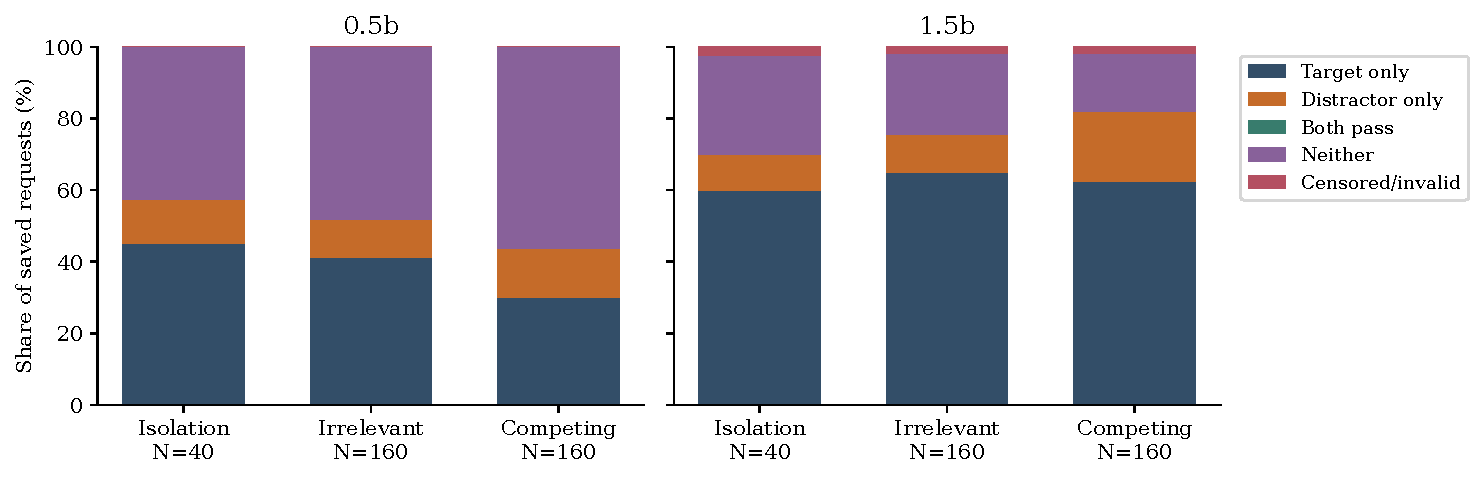
\includegraphics[width=.98\linewidth]{cross_outcomes.pdf}
\caption{Descriptive cross-specification cells. Isolation has 40 requests per
model; loaded groups have 160. Censored/invalid outcomes remain visible and
both-pass counts are explicitly zero. These stacked shares are not independent
request-level inferential estimates; paired effects use task means.}
\label{fig:cross}
\end{figure*}

Censoring limits this finding. Assigning every unknown competing response
against the association and every unknown control in its favor yields a 1.5B
difference of 6.88 points over all 40 tasks, scenario interval
$[-0.02,15.00]$, adjusted $p=0.53125$. The favorable assignment gives 10.62
points, interval $[3.75,18.75]$. These are adverse/favorable coding scenarios,
not observed repaired outcomes or a formal confidence set for missingness.
The complete-case result is therefore suggestive but not robust to all cap
assignments (Figure~\ref{fig:paired}).

\begin{figure*}[t]
\centering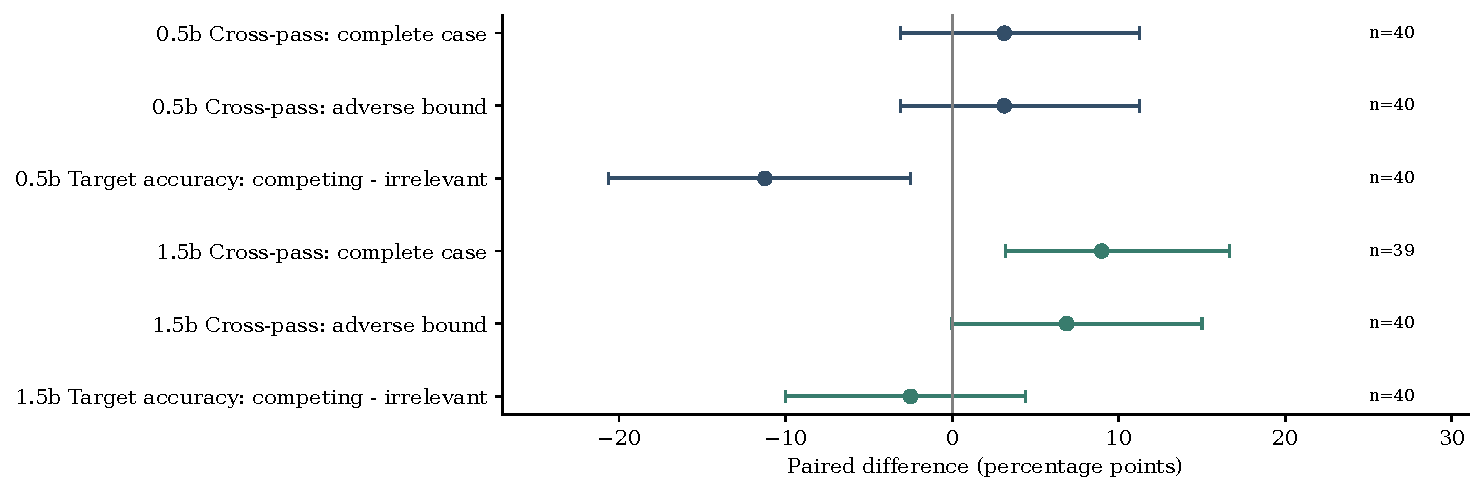
\includegraphics[width=.98\linewidth]{paired_effects.pdf}
\caption{Paired task effects for revised interference, with 95\% pointwise
bootstrap intervals. Cross-pass comparisons are posthoc. Adverse-bound rows
assign censored indicators against the observed association; target accuracy
uses registered bounded outcomes. Different endpoints and populations are
labelled rather than pooled.}
\label{fig:paired}
\end{figure*}

\subsection{Initial context load and static interruptions}
Initial context load shows a near-minus-irrelevant estimate of
\SmallInitialDiff{} points for 0.5B, interval \SmallInitialCI{}, Holm
$p=\SmallInitialP{}$, and \LargeInitialDiff{} for 1.5B, interval
\LargeInitialCI{}, $p=\LargeInitialP{}$. These selected populations and weaker
distractors cannot be pooled with the revised semantic experiment. Nor should
the numerically larger initial effect be taken as evidence of a stronger
internal capacity limit.

The six primary interruption comparisons do not establish a corrected effect.
For example, three other-domain descriptions versus neutral material on 1.5B
give $-15$ points with interval $[-27.5,-2.5]$, but Holm $p=0.421875$.
This illustrates the distinction between pointwise intervals and family tests.
Its constructed history and coarse domain labels also preclude a general claim
about real task switching. Isolated strategy differences are similarly
uncertain: P3\_1 minus P1 is \SmallPromptDiff{} points on 0.5B, interval
\SmallPromptCI{}, and \LargePromptDiff{} on 1.5B, interval
\LargePromptCI{}. These negative or inconclusive results constrain the narrative.

\section{Retention Policies and Computational Efficiency}
All five policies are shown in Table~\ref{tab:r1} and Figure~\ref{fig:r1}.
Oracle retention's correctness difference from full history is $+7.5$ points
on 0.5B, interval $[-5,22.5]$, and $+2.5$ on 1.5B, interval $[-10,15]$.
All six registered replay/oracle/compaction accuracy contrasts have Holm
$p=1$. Replay is not established to improve accuracy, and neither is
equivalent accuracy established by these wide intervals.

\begin{table*}[t]
\centering\small\begin{tabular}{llrrrr}
\toprule
Model & Policy & Correct/40 & Input & Output & Net mWh/correct \\
\midrule
0.5B & Full history & 14/40 & 1327.8 & 448.4 & 325.38 \\
0.5B & Target/query & 19/40 & 170.6 & 501.2 & 157.52 \\
0.5B & Verbatim replay & 15/40 & 1467.8 & 225.2 & 226.92 \\
0.5B & Lossless compaction & 16/40 & 177.0 & 193.7 & 79.29 \\
0.5B & Oracle retention & 17/40 & 183.6 & 196.0 & 76.39 \\
\midrule
1.5B & Full history & 22/40 & 1327.8 & 69.1 & 154.16 \\
1.5B & Target/query & 28/40 & 170.6 & 301.6 & 161.21 \\
1.5B & Verbatim replay & 23/40 & 1467.8 & 75.2 & 163.53 \\
1.5B & Lossless compaction & 22/40 & 177.0 & 64.6 & 53.00 \\
1.5B & Oracle retention & 23/40 & 183.6 & 63.6 & 50.20 \\
\midrule
\bottomrule
\end{tabular}

\caption{R1 observed outcomes, 40 tasks per policy/model. Tokens are means.
Energy is HWiNFO estimated net CPU-package mWh per correct solution, including
failed-attempt energy. All 40 requests have readings in each row. Confidence
intervals and paired contrasts are reported separately.}
\label{tab:r1}
\end{table*}

The measured cost contrast is much larger than the uncertain accuracy contrast.
Estimated net energy per correct solution is \SmallFullEnergy{} mWh for full
history and \SmallOracleEnergy{} for oracle retention on 0.5B; corresponding
1.5B values are \LargeFullEnergy{} and \LargeOracleEnergy{} mWh. These ratios
correspond to observed estimated-cost reductions of \SmallEnergyReduction\%
and \LargeEnergyReduction\%, computed as $100(1-C_{\rm oracle}/C_{\rm full})$.
They are descriptive reductions, without an established accuracy-preservation
guarantee. Paired
oracle-minus-full ratio differences are \SmallEnergyDiff{} mWh, interval
\SmallEnergyCI{}, and \LargeEnergyDiff{} mWh, interval \LargeEnergyCI{}.
These intervals resample complete paired task clusters and recompute both
ratios; they are not intervals on the energy of successful requests alone.

\begin{figure*}[t]
\centering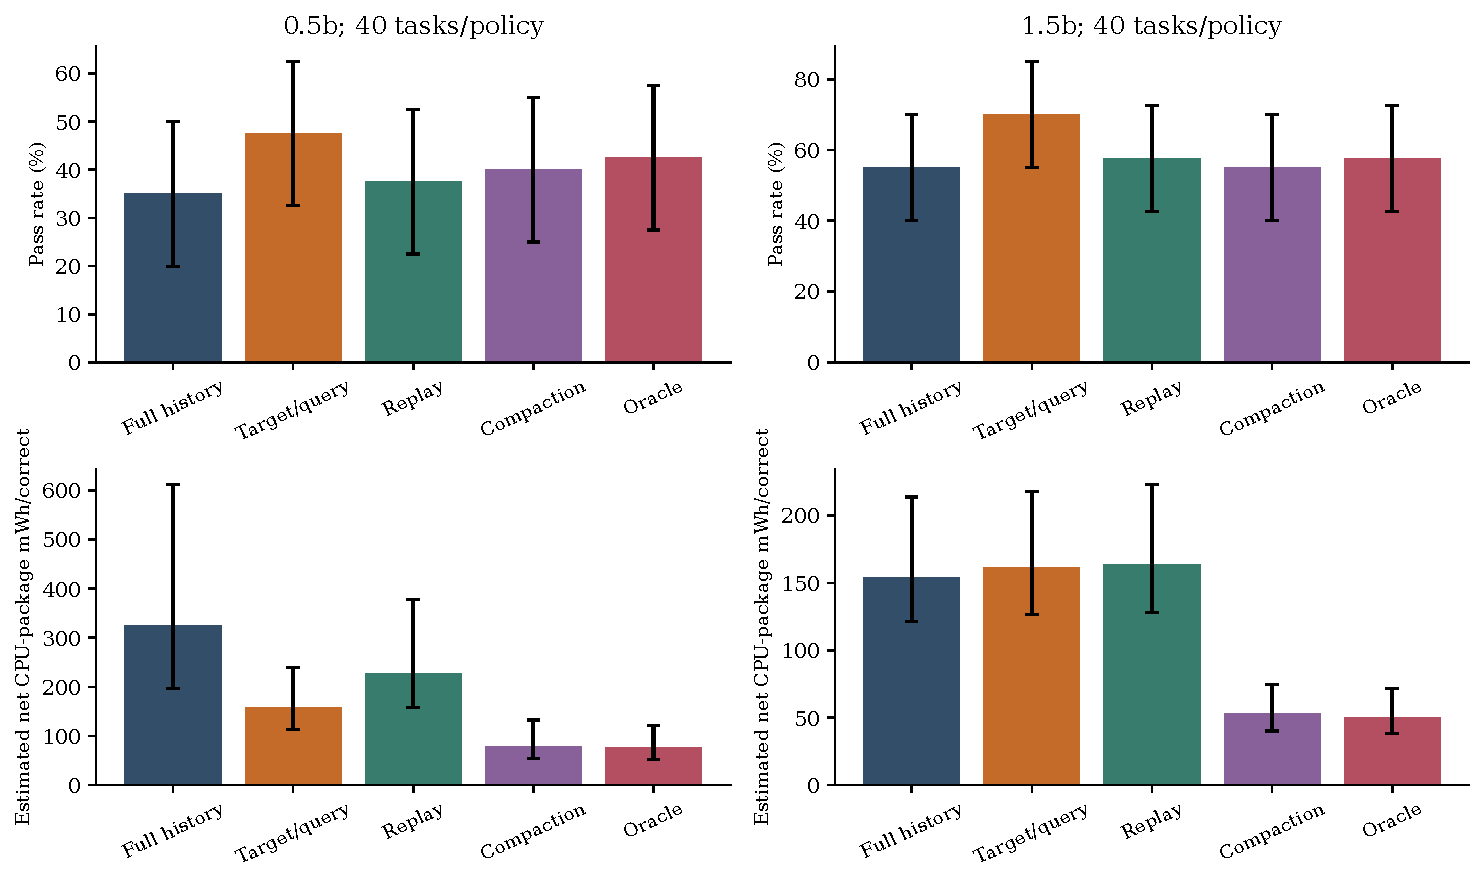
\includegraphics[width=.93\linewidth]{r1_policies.pdf}
\caption{R1 correctness and estimated net CPU-package energy per correct
solution, with pointwise task-bootstrap intervals. A shorter retained prompt
does not isolate memory-policy quality: instructions, input position and output
length also differ. Ratios include every covered attempt's energy. Model panels
use common scales within each row; target/query omits the code-only preference.}
\label{fig:r1}
\end{figure*}

End- and midpoint-baseline subtraction retain the lower oracle cost estimates
in these data. Excluding drifted observations also retains the direction, on
smaller matched populations. Cap exclusion reduces the 0.5B paired difference
to approximately $-112.65$ mWh over 35 tasks. Some short-window-excluded 0.5B
ratio draws have zero correct solutions; finite intervals are deliberately
left unavailable. In 1.5B oracle retention, removing short windows leaves only
18 of 40 calls. It preferentially removes cheap requests, rather than producing
a cleaner estimate for the original population.

Several alternatives remain. Oracle selection knows what matters, unlike a
deployed retriever. Full history and the reduced policies differ in input
length and recency. No-history omits the code-only instruction and produces
more output tokens; compaction only changes formatting of retained target text.
Generation budgets, output caps and runtime overhead can also influence ratios.
No automated retrieval/indexing cost is included. The sample Pareto display
(Figure~\ref{fig:pareto}) summarizes observed policy trade-offs, not a
population-optimal frontier or proof of accuracy-preserving energy savings.

\begin{figure*}[t]
\centering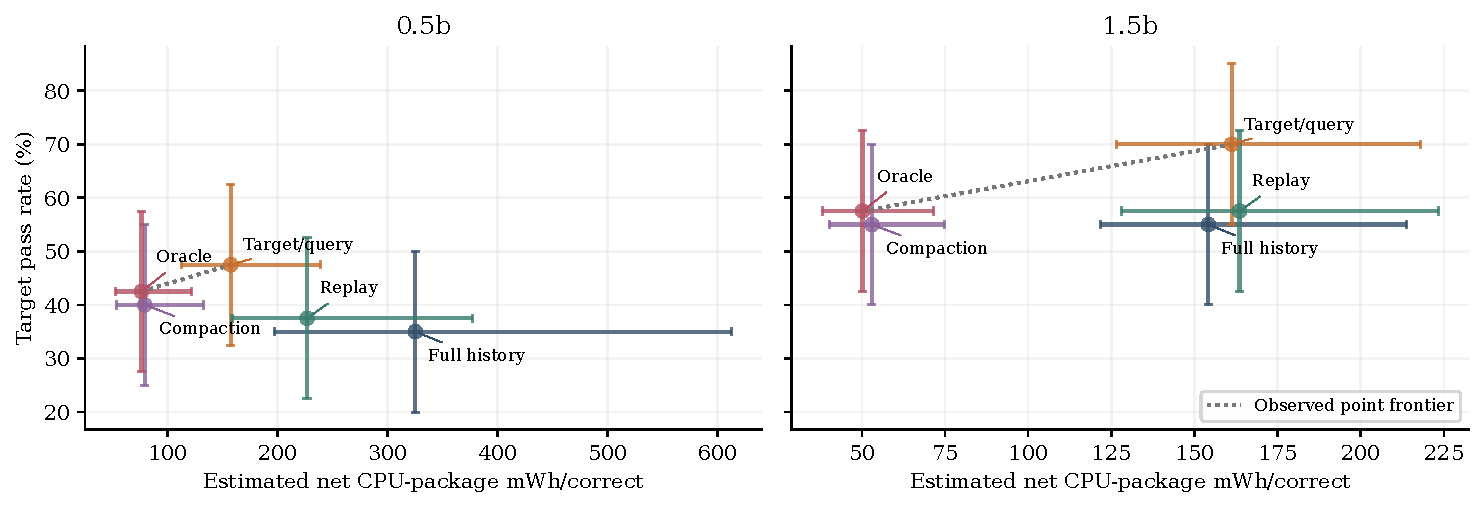
\includegraphics[width=.98\linewidth]{pareto.pdf}
\caption{Descriptive R1 accuracy--energy plots, separately by model, 40 tasks
per policy. Energy is HWiNFO estimated net CPU-package mWh/correct. Horizontal
and vertical whiskers are marginal bootstrap intervals, not joint confidence
regions. Both model panels share the same axes. The dotted frontier uses
sample point estimates only.}
\label{fig:pareto}
\end{figure*}

\section{Preference Utilization}
The registered adherence predicate requires unfenced parseable Python defining
the target function. It scores zero out of 400 full-study responses, so both
primary placement/reminder contrasts are at the observed floor. The instruction
asks for code only but does not explicitly prohibit Markdown fences. Treating
this floor as evidence that the model forgot every preference would therefore
overstate what the instrument measures.

A separate posthoc audit preserves the original scores and records fences,
outside prose, comments, docstrings and a fence-tolerant syntax predicate.
For 1.5B, each explicit-preference condition has 40/40 fence-tolerant outputs,
whereas no-preference has 21/40. For 0.5B, explicit conditions range from
36/40 to 39/40, versus 15/40 without the preference. These descriptive
differences do not establish long-term retention: immediate, buried and replayed
conditions also differ in rendered wording and position, and the registered
strict contrasts remain unchanged. Buried/replay comparisons under the
fence-tolerant predicate do not establish a benefit after correction.

Comments and docstrings can be legitimate code or explanatory content.
Mechanical counts do not replace human semantic adherence annotations. Joint
correctness-and-adherence outcomes are provided under each definition rather
than silently selecting the most favorable score. A zero-width empirical
bootstrap interval at an all-zero/all-one sample is not certainty about a
population rate. This scoring-definition problem is itself an honest limitation
of the experiment.

\section{MemoryGraph Companion Prototype}
\subsection{From Oracle Retention to Practical Memory Retrieval}
The existing MemoryGraph implementation is audited at commit
\texttt{c569143ec6be1c767a2c56c59c936f85bd1fc1cb}. It stores editable local
plain-text memories; TF-IDF and pretrained sentence embeddings rank candidates.
A NetworkX bipartite graph links memories to a small fixed entity vocabulary.
Its graph-assisted method adds a bounded bonus to lexical scores for shared
entities. This is not full GraphRAG, automatic memory extraction, or learned
feedback adaptation. Logistic regression and random-forest pipelines are
evaluation baselines, not a demonstrated learned online memory controller.

The interface exposes selected text and requires explicit approval before a
local Ollama response comparison. Limited warnings detect explicit pytest versus
unittest and VS Code versus PyCharm preference conflicts; they do not resolve
arbitrary contradictions. No usability, trust, personalization or energy benefit
was measured. Figure~\ref{fig:mg} describes the existing components only.

\begin{figure*}[t]
\centering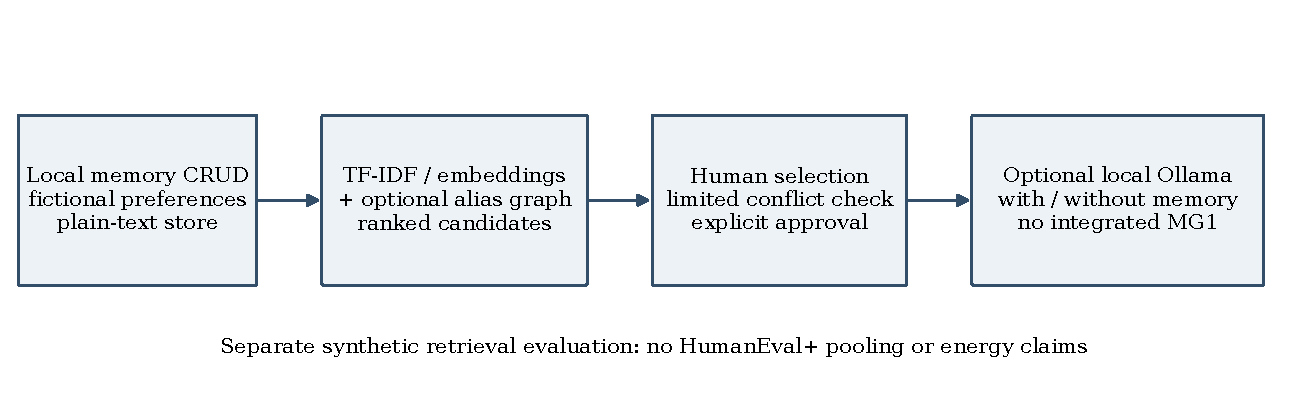
\includegraphics[width=\linewidth]{memorygraph_architecture.pdf}
\caption{Existing companion prototype, not an evaluated intervention in the
main study. Candidate selection and approval precede optional inference. The
separate saved synthetic benchmark evaluates ranking only; MG1 remains unrun.}
\label{fig:mg}
\end{figure*}

Its saved synthetic evaluation contains 600 labelled query--memory pairs,
24 fictional profiles and 120 queries with five candidate memories each.
Exactly one candidate is labelled relevant. Recomputed embedding MRR is
\EmbeddingMRR{}, versus \LexicalMRR{} for TF-IDF, using the saved scores and
stable tie ordering. The embedding snapshot and data hashes are retained.
The offline lexical benchmark fits its vocabulary across the saved corpus;
the interactive lexical retriever instead fits the query and candidate memories.
The benchmark MRR therefore does not directly measure the interface's ranking.
These are template-based synthetic rankings, not held-out code-generation
outcomes or estimates of real-user behavior. Grouped classifier evaluation
splits by fictional profile, but repeated templates can still supply shortcuts;
the random forest's recorded perfect synthetic result should not be read as
general memory-understanding ability.

A recorded two-prompt local demonstration supplies a pytest preference, yet
the memory-enabled response begins with \texttt{import unittest}. Both
successful API responses reach the 128-token output budget, and correctness
and energy were not scored. A preceding failed demonstration run is retained separately. This is a concrete example of availability without the intended
surface behavior, not a controlled integrated benefit or failure-rate estimate.
The HumanEval+ study and this synthetic benchmark are never pooled. An
integrated MG1 comparison remains Version 2 work.

\section{Discussion}
\paragraph{Diagnosing what went wrong.}
A target pass/fail score collapses several different outcomes. Cross-specification
testing adds a useful distinction: some failures satisfy a known competing
requirement, while others satisfy neither tested contract. Isolation cross-scoring
checks how often alternative-consistent behavior already occurs without competing
context. The larger model's complete-case difference supports this diagnosis as
a useful behavioral endpoint; its censoring sensitivity limits the strength of
the empirical association. Recency, repeated exposure, pattern completion and
ordinary boundary errors are possible explanations, not mechanisms identified
by this experiment.

\paragraph{Retrieval is an intermediate outcome.}
A practical memory system needs relevant text to be selected, its conflicts and
priority to be resolved, and the generated answer to satisfy the current task.
Retrieval success evaluates the selection step. It does not establish that the
model applies the selected requirement: Figure~\ref{fig:worked} has the target
in view, and MemoryGraph's recorded demonstration has the pytest preference in
view but emits unittest. The latter is a capped illustration, not a population
estimate. A future integrated evaluation should report retrieval relevance,
target correctness, preference adherence and total cost separately, so that
good ranking cannot hide a downstream utilization failure.

\paragraph{Retention is also a computational decision.}
The observed oracle/full-history cost gap makes selective context management a
useful practical question, but it does not isolate the benefit of selecting
relevant memories. Shorter input changes prefill work; position and instructions
can change the response; output length and failed attempts change decode cost
and cost per correct solution. Privileged relevance information and omitted
retrieval/indexing overhead further separate the oracle from a deployed system.
Length- and instruction-matched interventions with end-to-end overhead would be
needed to attribute savings to retrieval policy itself. Our uncertain accuracy
differences do not establish a safe compression or retention rule.

\paragraph{What the null results contribute.}
Replay is not consistently beneficial in the registered comparisons, static
interruptions are inconclusive after correction, and E5's strict score reaches
a floor partly explained by its treatment of fences. These outcomes argue for
validating the measurement before choosing a memory policy. They also narrow
the next research step: test retrieval and generation together under matched
instructions, with a validated adherence rubric, rather than assume that more
retained context or a reminder must help.

\section{Limitations}
The results concern two small quantized models, one code benchmark and one CPU
laptop. Training-set exposure is unknown; benchmark familiarity is neither ruled
out nor inferred from a pass. Fixed task rosters, noisy eligibility selection,
one structural generation per cell and only three isolated stochastic samples
limit generalization. Shared functions connect M1 bundles and prevent robust
component-level intervals. The smaller-model effects need not predict larger
models, other quantizations, GPUs or cloud deployments.

The study is revised and partly exploratory. Registrations and dated amendments
are preserved, but the final synthesis and cross-specification audit are
posthoc. Local Git hashes support provenance, not independent public
timestamping. Family correction does not erase prior exploration. The separate
synthetic prototype benchmark is small and templated, with no user study.

Scoring depends on finite test suites, extraction and a Windows restricted
subprocess adapter. These controls are documented rather than described as a
complete adversarial sandbox. Alternative construction and similarity labels
are AI-assisted and authored; representative witnesses are not exhaustive
semantic validation. Adverse censoring weakens the principal cross-pass result.
No recognition, internal state or intentional giving-up measurement exists.

CPU-package estimates are not calibrated process-specific energy. Unrelated
work, shared baselines, clock/sampling gaps, thermal effects and approximate
post-load boundaries remain potential errors. Bootstrap intervals reflect task
variation, not measurement calibration or independent block errors. Short
requests are particularly difficult at 500 ms resolution. The incomplete
registered cache experiment prevents a completed primary energy claim.

\section{Conclusion}
Across seven studies, the useful distinction is between supplying information
and obtaining code that uses it as intended. Cross-specification testing makes
one class of failure visible: the 1.5B complete cases show more
alternative-consistent outputs under competing context, although adverse
censoring weakens the finding. Oracle retention has lower observed estimated
energy per correct solution, while accuracy preservation remains unresolved
and policy effects are confounded. E5 supplies an equally important negative
lesson: a preference metric at its observed floor cannot support the intended
retention claim. These results support evaluating memory selection, generated
behavior and total computation together. They do not establish an internal
memory mechanism or an integrated MemoryGraph benefit.

\section{Data and Code Availability}
The repository is \url{https://github.com/buildgit17626-ctrl/Memory-Under-Interference-}.
The final Version 1 artifacts are associated with the reserved Zenodo DOI
\href{https://doi.org/10.5281/zenodo.24500468}{10.5281/zenodo.24500468}
and the designated version-specific GitHub release URL:
\url{https://github.com/buildgit17626-ctrl/Memory-Under-Interference-/releases/tag/v1.0.1}.
The DOI is reserved; its registration and public accessibility have not been
confirmed. GitHub packaging release v1.0.1 distributes this approved manuscript Version 1.0.
The author will complete Zenodo publication separately. The artifacts supply code,
frozen designs, transformed raw journals,
per-task scores, numerical power/time samples, analysis tables and source/hash
mappings. Original raw evidence remains unchanged locally. Unnecessary local
paths and process/account metadata are removed only in public derivatives;
original/public hashes distinguish them. Full multi-sensor CSV mirrors are not
redistributed; the numerical CPU-package/time exports reproduce the included
energy integrations. They do not calibrate the sensor or reconstruct other
hardware channels. The archive is an analysis release, not a claim that its
sanitized files can resume the original frozen supervisor. Zenodo publication
is left to the author and is not performed by this GitHub handoff.

\section{Author Contributions and AI-Assistance Disclosure}
Dhruv Brahmbhatt contributed the research questions, design decisions, experiment
oversight and interpretation review. He is an IIT Madras student conducting
this work independently; institutional supervision, sponsorship and endorsement
are not claimed. AI assistance supported setup, autonomous Ollama execution,
harness and analysis coding, distractor construction, auditing, literature
organization and manuscript drafting. AI-generated constructions were subject
to the recorded reference/witness checks; AI assistance is not independent
scientific validation. Original report/data are licensed under CC BY 4.0 and original code
under MIT, with third-party notices retained.
\label{maintext:end}

\begingroup
\footnotesize
\setlength{\bibsep}{3pt}
\bibliographystyle{plainnat}
\bibliography{references}
\endgroup
\onecolumn
\appendix
\section{Registered Primary Contrasts and Request Inventory}
\begin{center}\small\begin{tabular}{lrrrr}
\toprule Study & Calls & API failures & Caps & Energy readings \\
\midrule
E0 & 1968 & 2 & 6 & 1966 \\
E5 & 400 & 0 & 8 & 400 \\
M1 & 1040 & 0 & 11 & 1040 \\
M2 & 400 & 0 & 1 & 400 \\
M3R2 & 1040 & 1 & 10 & 1038 \\
M3\_initial & 280 & 0 & 1 & 280 \\
R1 & 400 & 0 & 5 & 400 \\
\bottomrule
\end{tabular}
\end{center}
These are scheduled logical requests, not retry counts. Caps are bounded-outcome
nonpasses; API failures remain separately missing for valid-input accuracy.
Energy readings are approximate post-load CPU-package observations. The revised
interference study has one missing energy window in addition to its API failure.
Pilot and partial-diagnostic counts remain separate in the archive.

Internal IDs are retained here to connect the narrative to frozen protocols.
E0 is the isolated strategy comparison; initial M3 is selected-task context
load; M1 is task bundling; revised M3/R2 is semantic interference; M2 is static
return-to-task interference; R1 is retention; E5 is preference placement.
The table reproduces specified primary contrasts; it does not relabel the
posthoc synthesis as a confirmatory study. Full intervals, transition IDs and
sensitivity populations are in the machine-readable archive.
E5 rows use its original strict-adherence endpoint and four-test Holm family,
not the secondary fence-tolerant metric. All-zero paired differences yield
degenerate empirical bootstrap intervals; these are not proof of population
equivalence. M1's diagnostic/exploratory comparisons and E5 secondary
correctness contrasts are supplied in the archive rather than relabelled primary.
\small\begin{longtable}{p{.075\linewidth}p{.065\linewidth}p{.26\linewidth}rrp{.18\linewidth}r}
\toprule Study & Model & Contrast & $n$ & Diff. pp & 95\% CI pp & Holm $p$ \\
\midrule
E0 & 0.5B & P3\_1 minus P1 & 163 & -2.25 & $[-7.77, 2.86]$ & 0.44696 \\
E0 & 1.5B & P3\_1 minus P1 & 164 & 2.64 & $[-1.22, 6.30]$ & 0.44156 \\
Initial M3 & 0.5B & near-minus-irrelevant averaged length & 20 & -27.50 & $[-45.00, -10.00]$ & 0.033691 \\
Initial M3 & 1.5B & near-minus-irrelevant averaged length & 20 & -2.50 & $[-17.50, 12.50]$ & 1 \\
R1 & 0.5B & lossless\_compaction minus full\_history & 40 & 5.00 & $[-7.50, 17.50]$ & 1 \\
R1 & 1.5B & lossless\_compaction minus full\_history & 40 & 0.00 & $[-15.00, 15.00]$ & 1 \\
R1 & 0.5B & oracle\_selective minus full\_history & 40 & 7.50 & $[-5.00, 22.50]$ & 1 \\
R1 & 1.5B & oracle\_selective minus full\_history & 40 & 2.50 & $[-10.00, 15.00]$ & 1 \\
R1 & 0.5B & verbatim\_replay minus full\_history & 40 & 2.50 & $[-7.50, 12.50]$ & 1 \\
R1 & 1.5B & verbatim\_replay minus full\_history & 40 & 2.50 & $[-5.00, 10.00]$ & 1 \\
M3R2 & 0.5B & near-minus-irrelevant averaged cells & 40 & -11.25 & $[-20.62, -2.50]$ & 0.056396 \\
M3R2 & 1.5B & near-minus-irrelevant averaged cells & 40 & -2.50 & $[-10.00, 4.39]$ & 0.63525 \\
M2 & 0.5B & similar minus neutral & 40 & -12.50 & $[-25.06, 0.06]$ & 0.89844 \\
M2 & 1.5B & similar minus neutral & 40 & -2.50 & $[-12.50, 7.50]$ & 1 \\
M2 & 0.5B & other\_one minus neutral & 40 & -7.50 & $[-17.50, 0.00]$ & 1 \\
M2 & 1.5B & other\_one minus neutral & 40 & 2.50 & $[-10.00, 15.00]$ & 1 \\
M2 & 0.5B & other\_three minus neutral & 40 & -5.00 & $[-17.50, 7.50]$ & 1 \\
M2 & 1.5B & other\_three minus neutral & 40 & -15.00 & $[-27.50, -2.50]$ & 0.42188 \\
\bottomrule
\end{longtable}
\normalsize

The broad starting claims about load, replay and a possible recognition--generation
gap motivated the project but are not all tested by this release. Load contrasts
do not establish internal capacity; the revised retention design does not test
the original replay-rate phase diagram; and the unrun recognition/hint studies
cannot establish a know--do gap. Frozen hypotheses and amendments remain intact.

\section{Scoring, Censoring and Oracle Audit}
The audit re-extracts saved outputs using the frozen extractor and checks native
request/response measurements. Separate sandbox records cross-score 1,029
uncensored revised-interference outputs on their alternative suites, including
isolation and controls. Sixty capped per-function candidates and one merged
complete-fence candidate are scored separately; none changes the audited target
correctness outcome. This does not prove the extractor is optimal or justify
removing caps from the registered endpoint.

HumanEval/32's original oracle anomaly is retained, with an exclusion
sensitivity. Caps-as-missing and optimistic cap-pass scenarios preserve their
different denominators. Held-out eligibility sensitivity excludes the selecting
P1 sample0 from isolated-strategy comparison outcomes. The original all-task
primary estimates remain intact. Failure reasons and infrastructure-policy
outcomes are not silently converted into evidence about model knowledge.

The cross-pass complete-case comparison requires all four competing and
irrelevant cells per task. Adverse/favorable assignments bound unknown
indicators; their intervals describe assigned scenarios. The principal 1.5B
point estimate and significance are sensitive to that assignment. No claim of
missing-at-random censoring is made. Zero both-pass cells remain explicit.

\section{Energy Robustness and the Partial Cache Diagnostic}
Original block baselines, drift flags and time/power windows remain in the
export. Start, end and midpoint subtraction are reported separately. Excluding
drift or short windows changes the retained task population; paired cost-ratio
sensitivities require covered observations in both arms. Undefined ratio draws
are reported rather than silently discarded. Total-request and approximate
post-load estimates answer different measurement questions.

E4's original feasibility pilot stops at 10 of 20 planned requests because one
response ends short of its intended workload. A separately registered JSON-array
amendment completes a 20-call pilot, then saves 76 of 400 full requests. These
workloads and pilots are not pooled. The full run has 35 cold and 41 warm
requests. Native cached-token counters show zero for the cold requests and
positive counts for the warm requests; model residency, preparation and priming
are logged separately. Matching by model, prefix and repeat yields only six
pairs in total, spread sparsely across cells. Most cells have zero or one pair;
they do not support the planned cache-energy inference. Setup/priming energy
is outside measured requests. A setup-only paused intent is not a completed
measured generation. No full E3 or U-family outcome is substituted.

\section{Companion Implementation and Reproduction Boundaries}
The pinned MemoryGraph source snapshot includes local CRUD, ranking, a fixed
alias graph, two narrow conflict categories and approval-gated optional Ollama
comparison. The archived synthetic dataset, per-pair scores and per-query
rankings permit MRR recalculation without embedding inference. Classifier
pipelines use grouped fictional-profile validation; template shortcuts remain.
No model weights, private memories, real-user records or executable trained
classifier pickles are needed in the release.

The portable reproduction script verifies release hashes, logical-call counts,
key fields and the principal paired comparisons from public records. An optional
full audit rebuild uses the supplied analysis code and dependencies. Offline
verification does not launch Ollama or regenerate embeddings. Original frozen
commit identifiers and transformation mappings remain provenance references;
sanitized archive bytes have their own checksums.

\twocolumn
\section{Representative Rendered Prompts}\label{app:prompts}
These examples are selected saved requests for HumanEval/0 on 0.5B, not new
prompt variants. The system message is \texttt{You are a helpful coding assistant.}
The public \texttt{examples/} directory supplies the exact UTF-8 prompt strings,
full call keys, native token counts, decoding options and SHA256 values; those
strings also occur in the archived call journals. The R1 examples below are
complete. The longer R2 and E5 layouts explicitly mark editorial omissions;
their complete unabridged strings remain in the supplement.

\subsection{Oracle-retained target, preference and query (complete)}
\lstinputlisting[basicstyle=\ttfamily\scriptsize]{../examples/r1-oracle.txt}

\subsection{Target and query without the preference (complete)}
\lstinputlisting[basicstyle=\ttfamily\scriptsize]{../examples/r1-target-query.txt}
The difference is an actual instruction difference in the collected policies,
not a length-only intervention. It helps explain why an oracle/no-history
comparison cannot isolate relevance selection.

\newpage
\subsection{Competing-context request used in the worked example (abridged)}
\lstinputlisting[basicstyle=\ttfamily\scriptsize]{../examples/r2-layout-excerpt.txt}
Only repeated copies are elided here; the exact archived request contains all
of them. They are task descriptions without implementation bodies or hidden
tests. Repetition to fill the budget, task position and explicit distractor
labelling are part of the construction and constrain its interpretation.

\subsection{Immediate preference in the placement study (abridged)}
\lstinputlisting[basicstyle=\ttfamily\scriptsize]{../examples/e5-layout-excerpt.txt}
The omitted region contains the fixed earlier-task descriptions. The wording
asks for code without explanation and does not explicitly ban Markdown fences;
the registered strict score nevertheless rejects fenced responses.

\end{document}
